\chapter{Introduction} % =================================================================================
The human nervous system is divided into two parts: The \gls{cns}, which consists of the brain and the spinal cord, and the \gls{pns} which includes all of the nerves that branch out from the brain and spinal cord into the most distal areas of our body. The \gls{pns} is susceptible to be affected by peripheral neuropathies, which are common (prevalence of approximately 2.4 up to 14.8 \%, rising with age~\cite{Martyn1997EpidemiologyNeuropathy,Gregg2004PrevalenceSurvey}) and can result in deficiencies or restrictions of sensory or motor abilities. Diagnosis and assessment of peripheral neuropathies traditionally rely on neurological examinations, which might provide inconclusive results or are not amenable to deeply situated peripheral nerves. Recently, \gls{mri} of peripheral nerves gained popularity, termed \acrlong{mrn} (\acrshort{mrn}). A problem, however, is that as of today \acrshort{mrn} is qualitative because it is subjectively assessed by the radiologists. The use of \acrshort{mrn} images to extract potential quantitative biomarkers, such as cross-sectional area and nerve compartment volume ratio have been proposed~\cite{Kronlage2017,Felisaz2017MRNeuropathy.,Balsiger2018SegmentationApproach}. However, a prerequisite for calculation of such biomarkers is the segmentation of the \gls{pns}, which is expensive and tedious work for radiologists, has reproducibility issues, and is not always clinically feasible~\cite{Porz2014Multi-modalMachine,Gillies2016Radiomics:Data}. For this reason, we aim to segment the nerves of the \gls{pns} automatically from \acrshort{mrn} images, as an initial step towards obtaining biomarkers for clinical use.\\
This introductory chapter starts with the medical motivation, including an anatomical overview of the \gls{pns}, a listing of peripheral neuropathies, and the current state-of-the-art of diagnosis in Section~\ref{sec:intro_medical}. Section~\ref{sec:intro_mia} provides a short outline of medical image analysis and the segmentation problem, while  Section~\ref{sec:intro_mlearn} introduces machine learning, the fundamental methodology behind this thesis. Finally, the chapter is concluded by the elaboration of our hypothesis, and the aim and structure of this thesis.

\section{Medical Motivation} \label{sec:intro_medical} % ===========================================================================
\subsection{Anatomy}
Our nervous system is divided into two parts: The \acrlong{cns} (\acrshort{cns}), including the brain and the spinal cord, and the \acrlong{pns} (\acrshort{pns}), which comprises all of the nerves that branch out from the brain and spinal cord into the most distal areas of our body. In general, the \gls{pns} connects the \gls{cns} to all parts of the body. Both, the \gls{pns} and the \gls{cns} consist of efferent and afferent nerves. Efferent nerves transmit signals from the brain to the effectors, i.e., muscles and glands, of the different body parts. Afferent nerves transmit signals from the receptors to the brain. The \gls{pns} is split into the \gls{sns}, responsible for sensory input and motor output, and the \gls{ans} which controls involuntary responses to regulate physiological functions. Furthermore, the \gls{ans} is distinguished into the sympathetic and the parasympathetic divisions, which act antagonistically: While the sympathetic division is responsible for "flight-or-fight" functions (e.g., increasing of heart-rate and lung action, inhibition of stomach and intestinal function), the parasympathetic division promotes the "rest-and-digest" functions (e.g., body relaxes, buildup of reserves) of the body.\\
Figure~\ref{fig:subfig:anat_spinal} depicts how the \gls{pns} is connected to the \gls{cns}: Nerve rootlets, which are groups of axons, form a spinal nerve. Nerve rootlets, leaving the spinal cord ventrally, belong typically to motor nerves. Nerve rootlets belonging to sensory nerves typically enter the spinal cord dorsal. Figure~\ref{fig:subfig:anat_nerve} shows the cable-like structure of peripheral nerves. Each nerve contains many axons, also called nerve fibers, which are hierarchically bundled together. Groups of nerve fibers are surrounded by the first layer of connective tissue called the endoneurium. Multiple groups of surrounded nerve fibers bundled together, surrounded by another layer of connective tissue, called the perineurium, form a fascicle. Multiple fascicles but also blood vessels, surrounded by a final layer of connective tissue, called the epineurium, form a peripheral nerve. The blood vessels supply the nutrients. The nerves fibers can be myelinated or unmyelinated. Myelination acts as an insulator and increases the transmission velocity of neural signals.\\
Figure~\ref{fig:subfig:anat_sagittal} shows the main nerves of the \gls{pns} of the lower limb, and  Figure~\ref{fig:anat_axial} a cross-sectional view of the right thigh including the \gls{n.} ischiadicus. We chose to depict the nerves of the lower limb only because the \acrshort{mrn} images we work with are all taken from the anatomical region of the thigh (see Section~\ref{sec:materials}). Therefore, the MRN images include parts of the \gls{n.} ischiadicus, and typically the branching where it splits into \gls{n.} tibialis and \gls{n.} fibularis, proximal to the knee. After this section, we will refer to the \gls{n.} ischiadicus by its English name the \textit{sciatic nerve}.

\begin{figure}[htbp]
    \begin{minipage}[c][0.9\textheight][t]{.5\textwidth}
        \centering
        \vspace*{\fill}
        \subfloat[]
        {
            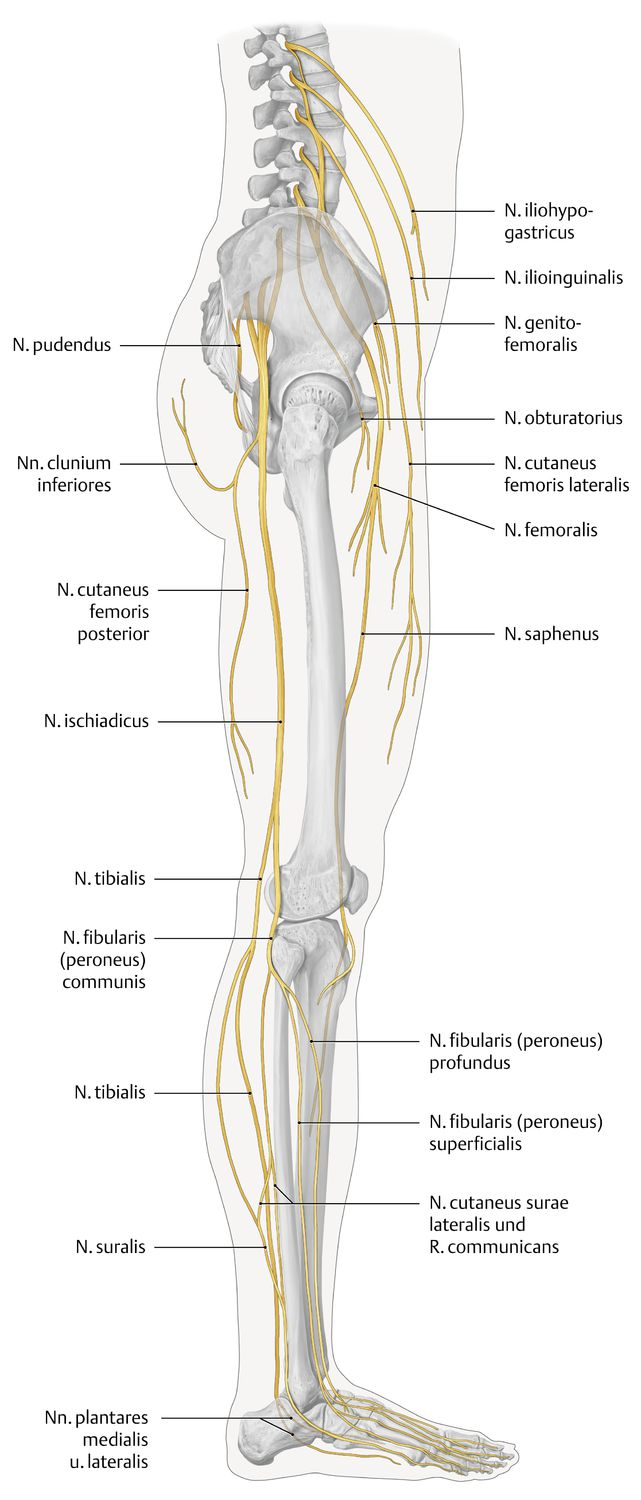
\includegraphics[width=\linewidth]{anat_sagittal}
            \label{fig:subfig:anat_sagittal}
        }
    \end{minipage}
    \begin{minipage}[c][0.9\textheight][t]{.5\textwidth}
        \centering
        \vspace*{\fill}
        \subfloat[]
        {
            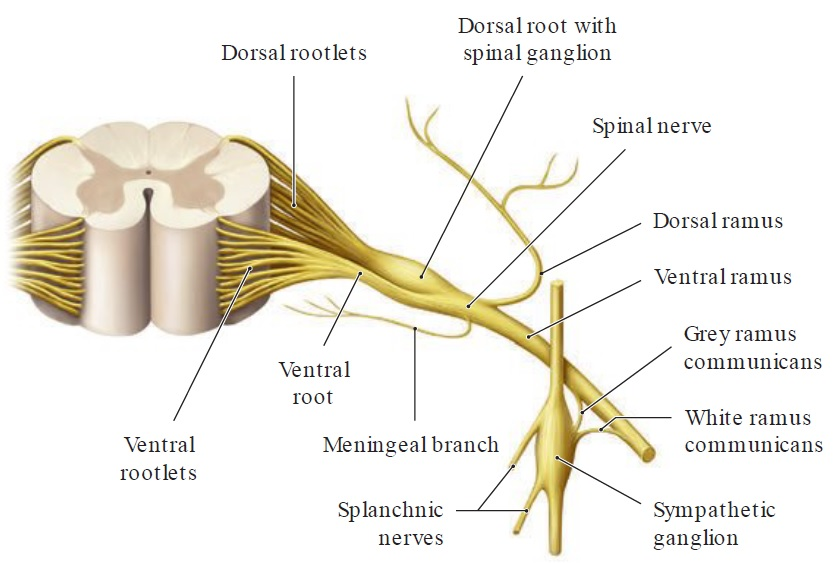
\includegraphics[width=\linewidth]{anat_spinal}
            \label{fig:subfig:anat_spinal}
        }
        \vfill
        \subfloat[]
        {
            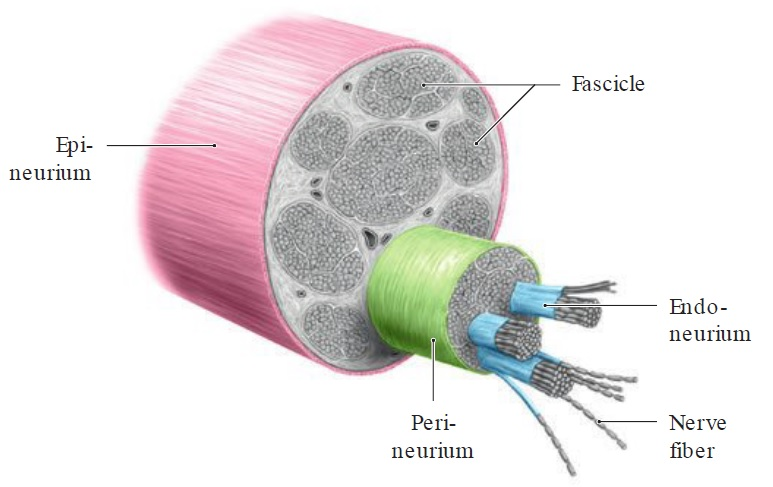
\includegraphics[width=\linewidth]{anat_nerve}
            \label{fig:subfig:anat_nerve}
        }
    \end{minipage}
    \vspace*{-0.3cm}
    \caption[Anatomy of the Peripheral Nervous System]{The anatomy of the \gls{pns} at different scales. \textbf{(a)} Nerves of the \gls{pns} of the lower limb, including the \gls{n.} ischiadicus. The \gls{n.} ischiadicus splits into the \gls{n.} tibialis and the \gls{n.} fibularis proximal of the knee.  \textbf{(b)} Sensory nerves enter the spinal cord dorsal and motor nerves exit the spinal cord ventral. \textbf{(c)} Structure of a peripheral nerve. Image \textbf{(a)} from~\cite{Schunke2014PrometheusAnatomie} and \textbf{(b)}, \textbf{(c)} from~\cite{Schunke2015THIEMEAnatomy}.}
    \label{fig:anat}
\end{figure}

\begin{figure}[htbp]
	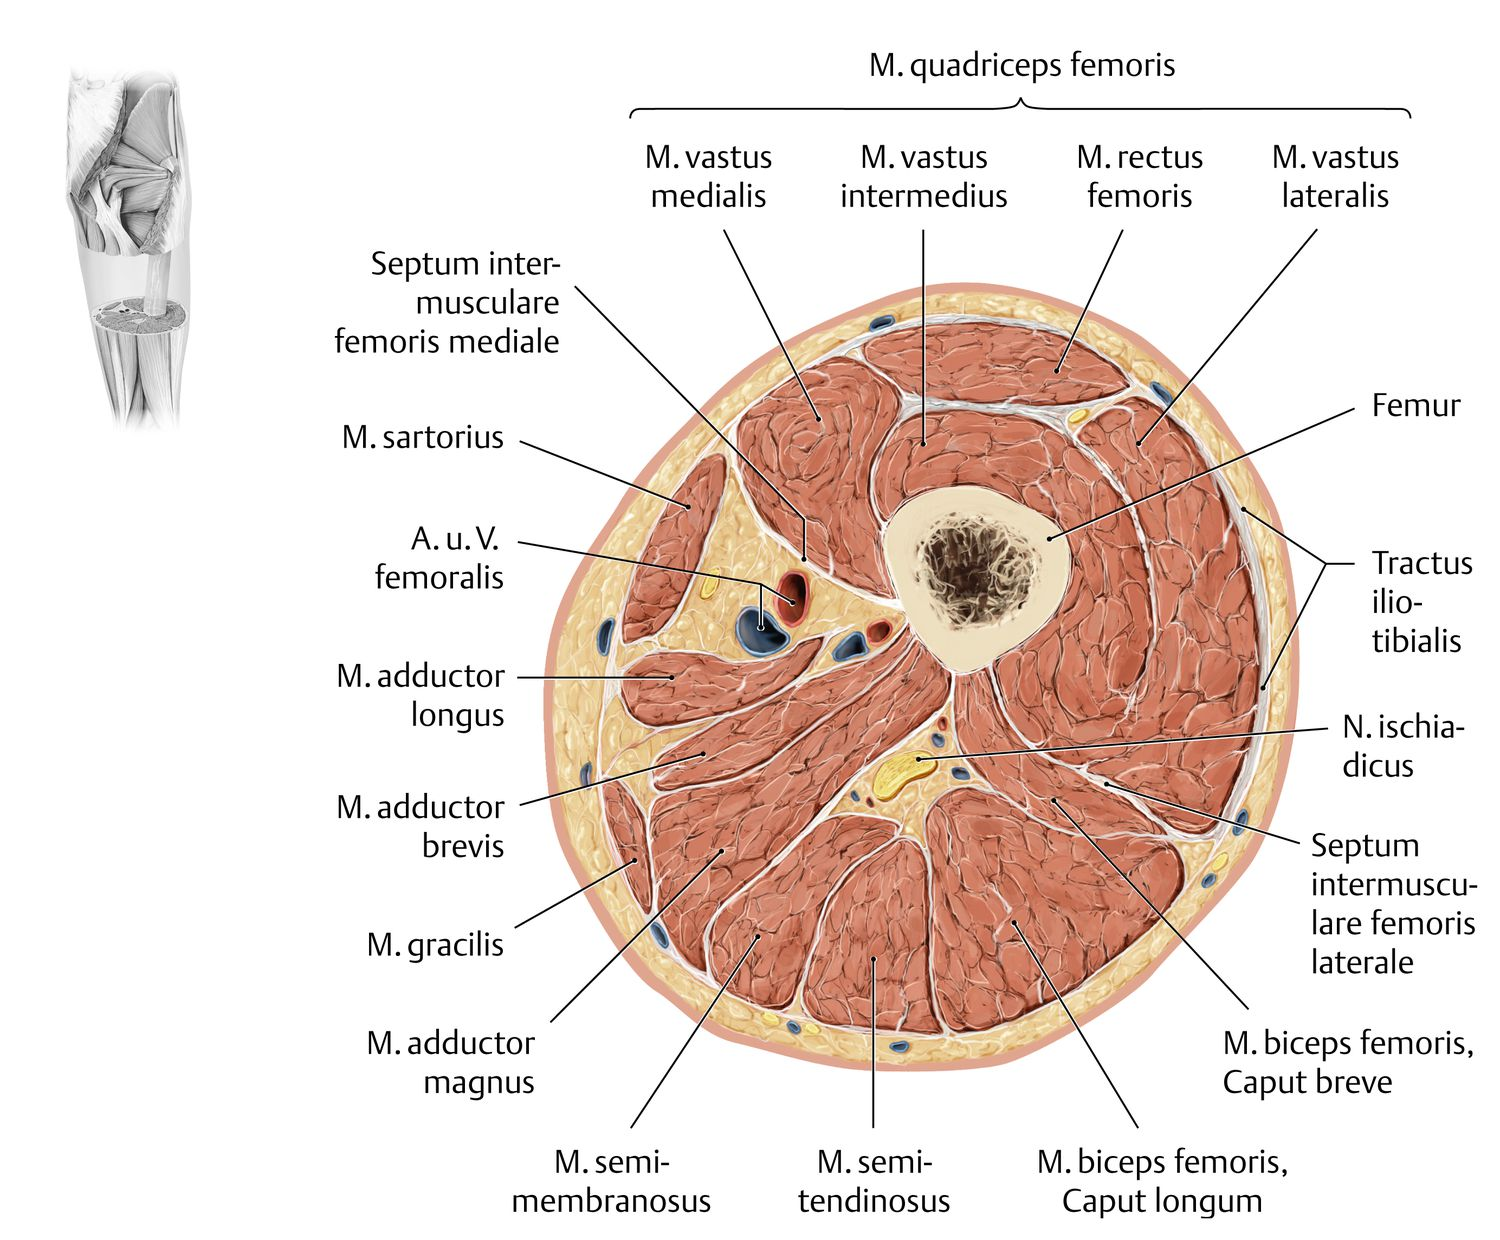
\includegraphics[width=\textwidth]{anat_axial}
    \caption[Cross-section of the Right Thigh]{Cross-sectional view of the right thigh with the femur, muscles, blood vessels, and \gls{n.} ischiadicus. Image from~\cite{Schunke2014PrometheusAnatomie}.}
    \label{fig:anat_axial}
\end{figure}

\subsection{Peripheral Neuropathies}
The prevalence of peripheral neuropathies is approximately 2.4 \% and rising to 8.0 \% with the age $\geq$ 55 years according to \cite{Martyn1997EpidemiologyNeuropathy}. A more recent study~\cite{Gregg2004PrevalenceSurvey} rises the prevalence of peripheral neuropathies with the age $\geq$ 40 years even to 14.8 \%. The most common cause of peripheral neuropathies in the developed world is diabetes mellitus. Other causes include metabolic disorders, infections, toxins, and drugs \cite{England2004PeripheralNeuropathy,Hughes466}.
Peripheral neuropathies can be caused by the damage of the axons or by demyelination, which hinders the fast transmission of neural signals. 
As the \gls{ans} controls almost every organ, a wide range of symptoms can arise when it is damaged. Damage to motor nerves may give rise to movement impairment or muscle weakness~\cite{Mohassel2015}. Damage to sensory nerves can be the cause of pain or altered sensation.

\subsection{State-of-the-Art Diagnosis}
Diagnosis and assessment of peripheral neuropathies rely on neurological examinations, which include clinical history, physical examination, and \gls{eds}. Biopsies, which are common in other medical fields, e.g., for the diagnosis or examinations of tumors and pathologies, are rarely conducted due to the irreversible damage to the nerves. \gls{eds} of the \gls{pns} are clinical tools that aid in the diagnostic assessment of patients with signs and symptoms of peripheral neuropathies~\cite{Mohassel2015}. \gls{eds} are used as an extension to the physical examination, and their primary goal is to help with the localization of peripheral nerve lesions and to assess their distribution (focal, multifocal, or generalized; one segment, multiple segments, or diffuse within the nerve)~\cite{Mohassel2015}. Additionally, \gls{eds} help determining age, severity, pathology, prognosis, and can be used for treatment planning~\cite{Mohassel2015}. Many physiologic and non-physiologic factors, e.g., age, height, tissue temperature, and pathology influence \gls{eds}. Normally, \gls{eds} are composed of two different tests, \gls{ncs} and \gls{emg}, which are related and complement each other.\\

\textbf{Nerve Conduction Studies}: \gls{ncs} measure the electrical signal propagation along a given nerve. The nerve of interest is stimulated at one site, and the electrical response signal is measured at another, which can then be analyzed. Typical signal measurements for \gls{ncs} include distal latency, amplitude, conduction velocity, and late response latency. Prolonged distal and late response latency, and reduced conduction velocity can indicate degeneration of the myelin sheath. A decreased amplitude can be the indicator of axonal degeneration~\cite{Mohassel2015}. However, a correct stimulation of proximal and deeper nerves is difficult. Therefore, those nerves are typically difficult to assess with \gls{ncs}~\cite{Mohassel2015}. \\

\textbf{Electromyography}: \gls{emg} or needle \gls{emg} complements \gls{ncs}, and can help to confirm suspected pathologic processes. \gls{emg} includes the evaluation of spontaneous activity at rest and the assessment of voluntary motor units upon activation by inserting a needle into the muscle. The needle serves as electrode and locally samples electrical activity of the muscle fibers. As \gls{emg} comes with discomfort for the patient (needle insertion), and a large number of muscles which could potentially be investigated, it is important to have a detailed anatomical knowledge and a hypothesis-driven approach~\cite{Mohassel2015}.\\
As of today, \gls{eds} are the first choice for the diagnosis of peripheral neuropathies. Apparent drawbacks are the insertion of the needle during \gls{emg} and that electrical stimulation may be painful or cause discomfort. Furthermore, \gls{eds} may not be applicable to nerves situated deep in the body, stimulate only the fastest conducting nerve fibres, and may yield inconclusive results.

\subsection{Imaging of the Peripheral Nervous System}
Imaging of the \gls{pns} as a complementary diagnostic tool to the state-of-the-art diagnosis has gained increasing attention in recent years. The following modalities are usually used to image the \gls{pns}~\cite{Ohana2014CurrentSystem}.\\

\textbf{\gls{us}}: \gls{us} can be used for examination because the nerves of the \gls{pns} usually are very superficial. Figure~\ref{fig:subfig:imag_us} shows \gls{us} images of the \gls{n.} ulnaris. \gls{us} is cheap and widely available. Advantages of \gls{us} are the large \gls{fov}, and that there are no contraindications. \gls{us} however, is very operator dependent and also suffers from poor contrast resolution of for the nerves. Furthermore, there are limitations to the applicability of \gls{us} in deep or difficult accessible anatomical areas~\cite{Ohana2014CurrentSystem}.\\

\textbf{\gls{mrn}}: \gls{mrn} is \gls{mri} tailored to the imaging of peripheral nerves. Optimized MR sequences allow for better contrast between the nerves and their surrounding tissues. Phased-array coils and high field imaging (e.g., 3~Tesla or higher) increase signal-to-noise ratio as well as the spatial resolution, allowing nerves to be examined. \gls{mrn} has excellent soft-tissue contrast and a higher \gls{fov} than \gls{us}. The resulting images are \gls{3d} and even deeply situated nerves can be imaged. Typically, the \gls{mrn} protocols make use of T1-weighted spin-echo sequences (excellent spatial resolution), T2-weighted spin-echo sequences (good contrast resolution), and "neurography" sequences, which are strongly T2-weighted using long echo times and fat signal suppression~\cite{Ohana2014CurrentSystem}. \gls{mrn}, however, is rather costly, has limited availability and acquisition may take a long time. Figure~\ref{fig:subfig:imag_mrn} depicts \gls{mrn} images of the \gls{n.} ulnaris at the wrist.\\

\textbf{\gls{ct}}: \gls{ct} is not as often used as the previous imaging modalities for peripheral nerves but it has some distinct benefits. \gls{ct} is useful in diagnosing spinal nerve compressions, and is often combined with \gls{ct} Myelography. \gls{ct} has a good spatial resolution, and excellent bone contrast. However, although large nerve trunks are often visible, the low contrast resolution does not enable a detailed examination of the neuronal microstructure~\cite{Ohana2014CurrentSystem}. Another disadvantage is the inherent irradiation of the tissue. Figure~\ref{fig:subfig:imag_ct} shows a curvilinear nerve reconstruction based on a \gls{ct} angiogram.\\


\begin{figure}[htbp]
	\centering
	\subfloat[]
	{
		\label{fig:subfig:imag_us}
		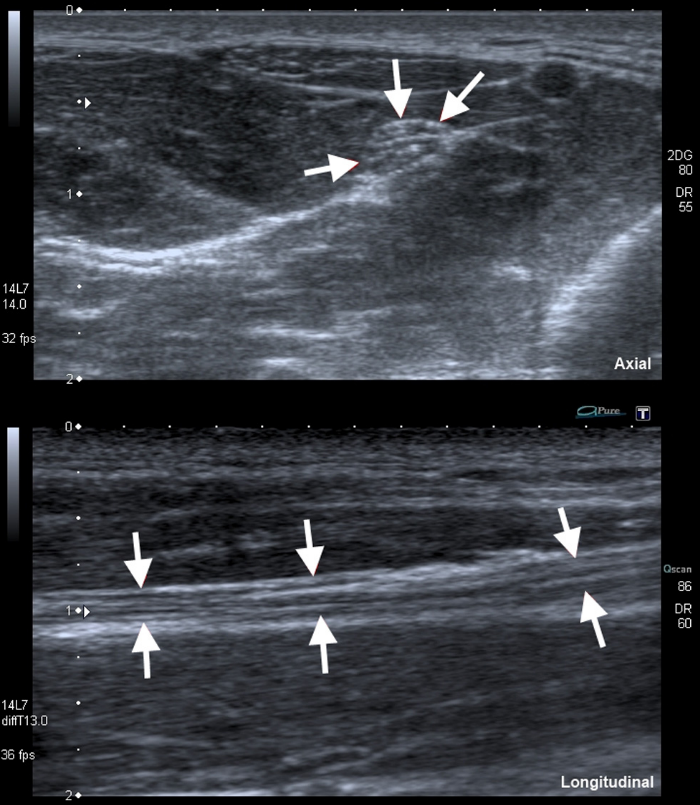
\includegraphics[width=0.48\textwidth]{imag_us}
	}
	\hfill
	\subfloat[]
	{
		\label{fig:subfig:imag_mrn}
		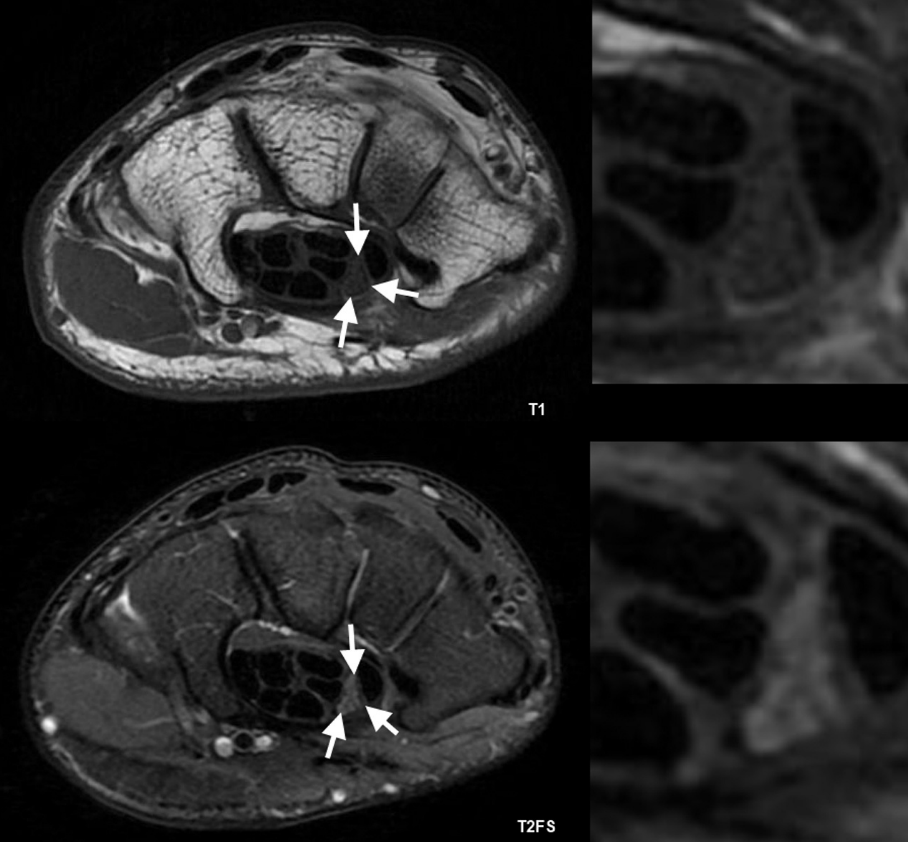
\includegraphics[width=0.48\textwidth]{imag_mrn}
	}
	\hfill
	\subfloat[]
	{
		\label{fig:subfig:imag_ct}
		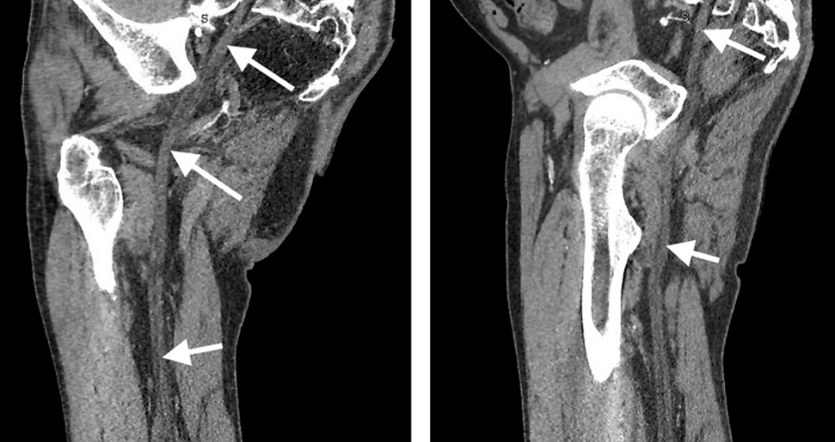
\includegraphics[width=0.7\textwidth]{imag_ct}
	}
	\caption[Modalities for Imaging of the Peripheral Nervous System]{Different modalities for \acrlong{pns} imaging. \textbf{(a)} \gls{n.} ulnaris at the wrist visible in axial (top) and longitudinal ultrasound sections. \textbf{(b)} Sagittal sections of the \gls{n.} medianus: T1-weighted image (top) and T2-weighted image with fat suppression (bottom). \textbf{(c)} Curvilinear reconstructions of the right \gls{n.} ischiaducus from a lower limb CT angiogram. Images from~\cite{Mohassel2015}.}
	\label{fig:imag_modalities}  
\end{figure}

\section{Medical Image Segmentation} \label{sec:intro_mia} % ===================================================================
Segmentation in digital image processing refers to the extraction of a target structure of interest from an image, or to partition the image into multiple segments. Segmentation results in a representation, which is easier to analyze. Typically, object boundaries or regions belonging to one semantic object are of interest. The task of segmentation, in essence, boils down to the pixel-wise assignment of object membership or more commonly class labels. Pixels belonging to the same object, i.e. share some characteristics, have the same class labels assigned.\\
Medical image segmentation usually involves the segmentation of an anatomical object of interest in some medical image, e.g., \gls{ct} or \gls{mri} image. The segmentation has to be performed manually by an expert due the required anatomical and image knowledge. Such manual segmentation is not always reproducible, means tedious work and is time-consuming. Even more so, by the fact that the medical images are often \gls{3d} images. Therefore, medical image segmentation is subject to research aiming at having automatic or semi-automatic, computer-assisted segmentation tools. However, such tools are not always able to deliver the required performance due to . Recently, deep learning-based segmentation of medical images, with the use of convolutional neural networks has become increasingly popular~\cite{Ronneberger2015U-Net:Segmentation,Tetteh2018DeepVesselNet:Volumes,Cicek20163DAnnotation,Baumgartner2017AnSegmentation,Meng2017TrackingNetwork,Milletari2016V-Net:Segmentation,BalsigerContext-awareNeurography,Kayalibay2017CNN-basedData}, and achieved or even surpassed human-level performances.

\section{Machine Learning} \label{sec:intro_mlearn} % =============================================================================
In this part, we briefly describe some fundamentals of machine learning. Machine learning is a huge topic and this section is by no means meant to be a complete overview. We rather introduce concepts and mention topics, which are related and important for our work.

\subsection{Supervised Learning} \label{sec:ml_supervised}
The principle of supervised learning is illustrated on the prediction of house prizes as a function of their living area in Figure~\ref{fig:dl_supervised}~\cite{Ng2012StanfordNotes}. In supervised learning, we train an algorithm (also called model) by providing the algorithm input-output pairs (e.g., living area of houses with their corresponding prizes). This is referred to as the training phase, and the input-output pairs are called the training set. The outputs are typically referred to as labels or targets. More formally, we define the training set as
\begin{equation}
   S_{Train} = \{(x^{(i)}, y^{(i)}); \quad i = 1,...,m\},
   \label{eq:training_set}
\end{equation}
where $(x^{(i)}, y^{(i)})$ denotes the $i$-th input-output pair consisting of the data $x$ and the label $y$. Let $\chi$ and $\upsilon$ denote the space of input and output values, respectively. In this example, $\chi = \upsilon = \mathbb{R}$. The aim of the training phase is to let the algorithm learn a meaningful relationship between the inputs and outputs of our training set. Therefore, we aim learn a mapping $h : \chi \mapsto \upsilon$, parameterized by a set of models weights~$\textbf{W}$, which is \textit{good} for all pairs in $S_{Train}$, hence
\begin{equation}
   y^{(i)} = h(x^{(i)}; \mathbf{W}); \quad i = 1,...,m,
   \label{eq:model}
\end{equation}
is approximatively valid for all training pairs. We call $h(x^{(i)}; \mathbf{W})$ our model, parameterized by the model's weights~$\textbf{W}$. Depending on the type of mapping, $\mathbf{W}$ is typically a matrix and we therefore, write it in bold capital letter. If the training is able to find a meaningful relation, the model can be used to make predictions on previously unseen input data $\hat{x}$.\\
If the output, we are trying to predict, is continuous, such as in the housing example, the problem is called a \textbf{regression problem}. We could also have the situation where we wanted to predict whether the dwelling is an apartment or a house, given the living area. The predicted output would, therefore, be discrete and we would call this a \textbf{classification problem}.\\
Supervised learning gets its name for the reason that the algorithm always learns on input-output pairs. Typically, the outputs  are the result of (laborsome) labeling work done by a person. This is the largest drawback of supervised learning. There exist ways to use unlabeled data in conjunction with labeled data, referred to as semi-supervised learning. Learning on input data without labels corresponds to finding patterns and structures in the input space and is referred to as unsupervised learning. Typical examples for unsupervised learning algorithms are \gls{pca} and $k$-means clustering~\cite{Goodfellow2016DeepLearning}.\\
For the housing example, one could expect a linear relationship, between the living area of a house and its prize. If this was indeed true, we could make robust predictions with a simple linear model, i.e. $y^{(i)} = h(x^{(i)}; W) = Wx^{(i)} + b$, only incorporating the living area. Note that in this case, the parameters of our model are a single scalar weight $W$ and a bias term $b$.
However, one could argue that the number of rooms or the location, each with its unknown weight, also influence the dwelling's prize. These influences are typically called features. There was and still is a whole science around finding good features to solve learning problems, which often relied on hand-crafting these features. The main drawback of any learning algorithm relying on hand-crafted features is that the algorithm is inherently constrained by the imagination and ability of the engineer to find and implement good features.

\begin{figure}[htbp]
    \centering
	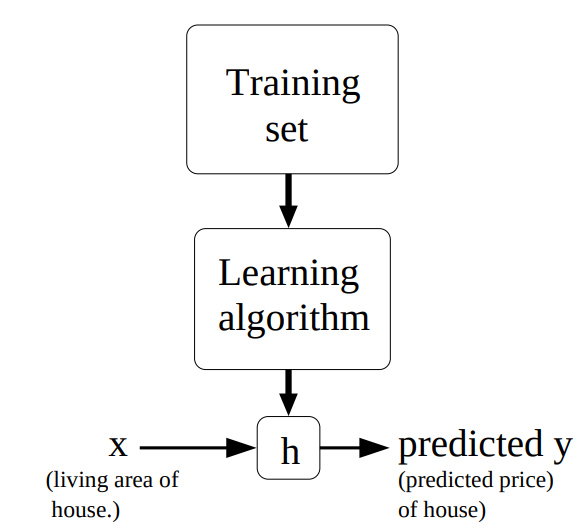
\includegraphics[width=0.5\textwidth]{supervised_learning}
    \caption[Supervised Learning]{The principle of supervised learning illustrated on the example of predicting house prices y depending on the living area x. Suppose we have $m$ area-price pairs, which we name our training set: $\{(x^{(i)}, y^{(i)}); \quad i = 1,...,m\}$. We let $\chi$ and $\upsilon$ denote the space of input and output values, respectively. In this example, $\chi = \upsilon = \mathbb{R}$. In supervised learning we aim to learn a function (also called mapping) $h : \chi \mapsto \upsilon$, which makes reasonable prize prediction y for a given new house area $\hat{x}$. We use the training set to learn $h$. Image and example taken from~\cite{Ng2012StanfordNotes}.}
    \label{fig:dl_supervised}
\end{figure}

\subsection{Training}
In the previous section, we defined that the model $h(x^{(i)}; \mathbf{W})$ is parametrized by the set of weights $\textbf{W}$. During the training phase of the model, we adjust $\textbf{W}$ in order for the model to make better predictions on the training set. Formally, we want to solve the optimization problem
\begin{equation}
   \mathbf{W}^{*} = \argmin_\textbf{W} \sum_{i=1}^{m} L(h(x^{(i)}; \mathbf{W}), y^{(i)}),
   \label{eq:optimization}
\end{equation}
where $L(\cdot)$ denotes a loss function. The loss function is a metric we have to choose, which calculates the error between the correct label $y^{(i)}$ and the prediction $\hat{y}^{(i)}$ our model made. The loss function is often also referred to as cost function. $\mathbf{W}^{*}$ denotes the solution for the mentioned optimization problem and, consequently, is the set of weights which results in the smallest error in our training set. Training of a model corresponds to iteratively decreasing the training error.\\
A loss function typically used for classification problems with $k$ classes, a prediction vector $\mathbf{h}^{(i)} \in \mathbb{R}^k$ and a categorial label vector $\mathbf{y}^{(i)} \in \{0,1\}^{k}$, is the \textbf{cross-entropy} loss

\begin{equation}
    L(\mathbf{h}^{(i)}, \mathbf{y}^{(i)}) = -\sum_{c=1}^{k}\mathbf{y}_{c}^{(i)} \log(f(\mathbf{h}^{(i)})_c),
    % L(\mathbf{h}^{(i)}, \mathbf{y}^{(i)}) = -\mathbf{y}^{(i)} \log(f(\mathbf{h}^{(i)})),
    \label{eq:cross_entropy_multi}
\end{equation}
with $f(\cdot)$ being the \textbf{softmax} function
\begin{equation}
   f(\mathbf{h}^{(i)}) = \frac{\exp\mathbf{h}^{(i)}}{\sum_{j} \exp{\mathbf{h}^{(i)}_{j}}},
   \label{eq:softmax}
\end{equation}
which squashes the predictions into a vector of values between zero and one that sum to one. The corresponding cross-entropy loss for a binary classification problem is
\begin{equation}
    L({h}^{(i)}, {y}^{(i)}) = -{y}^{(i)} \log(\sigma({h}^{(i)})) - (1- {y}^{(i)})\log(1- \sigma({h}^{(i)}))
    %L({h}^{(i)}, {y}^{(i)}) = -{y}^{(i)} \log(\sigma({h}^{(i)}))
    \label{eq:cross_entropy_binary}
\end{equation}
with $\sigma(\cdot)$ being the \textbf{sigmoid} function
\begin{equation}
   \sigma({h}^{(i)}) = \frac{1}{1 + \exp{(-{h}^{(i)})}}.
   \label{eq:sigmoid}
\end{equation}

In order to solve Equation~\ref{eq:optimization}, optimizers are used. Optimizers, such as \gls{sgd}~\cite{Goodfellow2016DeepLearning} and Adam~\cite{Kingma2014Adam:Optimization} use the gradient to find $\textbf{W}^*$. The gradient depends on the model and the chosen loss function, and corresponds the first-order derivatives of the individual inputs with respect to the outputs.\\

A common problem in machine learning is under- and overfitting (Figure~\ref{fig:under_over_fitting}). To solve a learning problem, we have to choose a model first. The model's representational power, hence the ability to fit a wide variety of functions, is called capacity~\cite{Goodfellow2016DeepLearning}. If the model's capacity is too low for the task at hand, it cannot model the relationship between the input and output. This is called underfitting. On the contrary, if the models capacity is too high, it can start to memorize the data it was trained upon (including the data's statistics) rather than learning structures or relationships. This results in a bad performance on new, unseen data, hence bad generalization, which is called overfitting.

\begin{figure}[htbp]
    \centering
	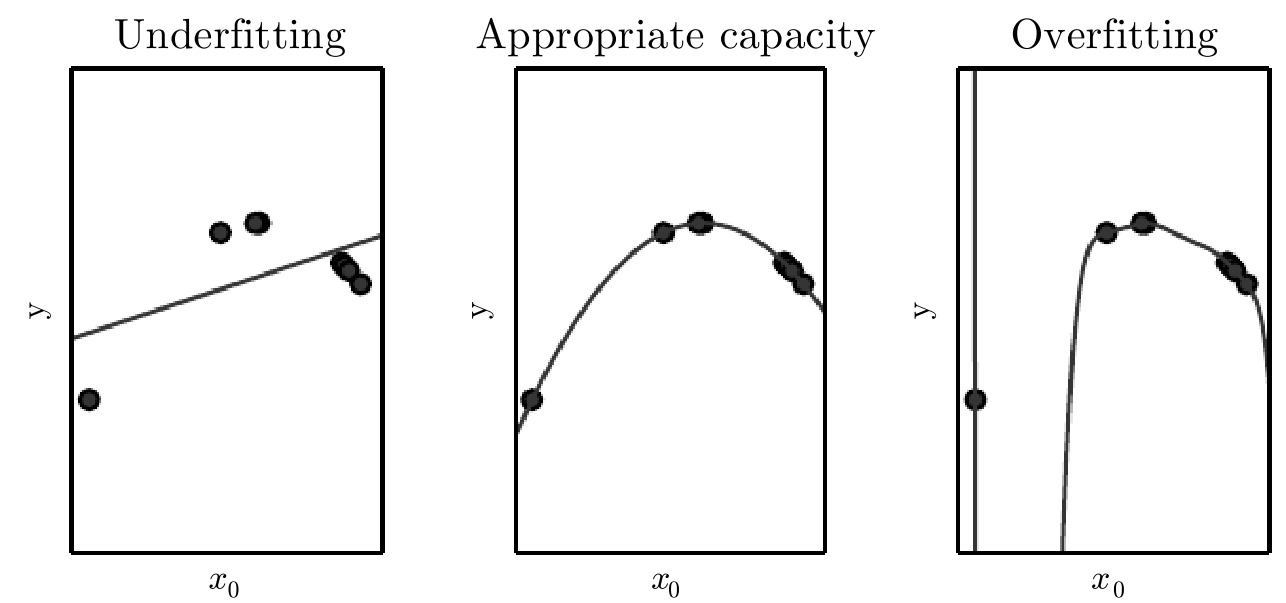
\includegraphics[width=0.8\textwidth]{under_over}
    \caption[Under- and Overfitting]{The problem of under- and overfitting of machine learning algorithms. The points were generated by random sampling a quadratic function. In the left image, a model with low capacity (a line) is not able to correctly capture the structure of the points. The center image shows that a quadratic model would generalize well to unseen points. The right image shows that a 9\textsuperscript{th} degree polynomial would generalize bad to new points despite passing through all points. Image and example taken from~\cite{Goodfellow2016DeepLearning}.}
    \label{fig:under_over_fitting}
\end{figure}

\subsection{Deep Learning \& Convolutional Neural Networks}
With the growing amount of labeled data, gathered in large datasets, and increasing computational performance using \gls{gpu}s, the creation and training of models, called neural networks, with much larger capacity became possible. The most significant advantage of those models was that (given enough training data) it was now possible to train them directly on raw, unprocessed data, rather than on human-engineered features.\\
\gls{cnn}, a class of neural network mostly used to analyze visual imagery, achieved new levels of performances in computer vision tasks and challenges \cite{Krizhevsky2012ImageNetNetworks,Simonyan2014VeryRecognition,Szegedy2014GoingConvolutions,He2015DeepRecognition,Zeiler2014VisualizingNetworks}. 
CNNs and neural networks in general, use a cascade of multiple layers of units which can process and transform data. Each layer takes the previous layer's output as an input. \gls{cnn}s, in contrast to regular neural networks, assume that the input data has some spatial relationship, hence the popular use of \gls{cnn}s for computer vision tasks. Because a \gls{cnn} consists of several sequential convolutional layers, the learned filters deeper in the network can act as detectors for higher semantical features. Therefore it can learn multiple levels of representations, which correspond to multiple levels of abstraction. During training, a \gls{cnn} learns the convolutional filters, which act as detectors for features present in the data. It basically builds its internal filter bank to extract information. Figure~\ref{fig:mlearn_weights} shows the learned filters in the first layer of an AlexNet trained for natural image classification~\cite{Russakovsky2015ImageNetChallenge}. Note that the learned weights resemble filters for edge or blob detection (sobel operator~\cite{Sobel1990AnOperator}, Laplacian of Gaussian~\cite{Marr187}) widely used in computer vision.\\
A typical \gls{cnn} is built as a sequence of multiples of the following layers~\cite{KarpathyStanfordRecognition}. Each layer transforms the activations of the previous layer into new activations, through a differentiable function.\\
We briefly summarize the most used type of layers.

\textbf{Convolutional Layer:} Layer which contains the learnable weights. The learnable weights form filters, which are used for information extraction. Parameters for a convolutional layer are typically the kernel size of the filters and the number of individual filters (also referred to as channels or features).\\

\textbf{ReLU Layer:} Applies the Equation~\ref{eq:relu} to each of the outputs of the previous layer. This results in thresholding at zero. Other typical activation functions are the sigmoid (Equation~\ref{eq:sigmoid}) or the tanh function.\\
\begin{equation}
   ReLU({h}^{(i)}) = \max(0, {h}^{(i)}).
   \label{eq:relu}
\end{equation}

\textbf{Pooling Layer:} A pooling layer performs a down-sampling operation along the spatial dimensions. Typically max-pooling is used, which only lets the maximum activation through. Pooling helps prevent overfitting by reducing the number of parameters in a network.\\

\textbf{Transposed Convolutional Layer:} A transposed convolutional layer performs and up-sampling operation along the spatial dimensions and is typically used as the inverse operation of the pooling layer.\\

\textbf{Dropout layer:} Randomly deactivates some of the activations of the previous layer. Dropout~\cite{Srivastava2014Dropout:Overfitting} is a type of regularization and thus aims to reduce the overfitting problem.\\

\textbf{Normalization Layer:} Different types of normalization layers have been proposed, including Batch Normalization~\cite{SergeyIoffe2015BatchNormalization}. They all normalize the activations in some way.
 
\begin{figure}[htbp]
	\centering
	\subfloat[]
	{
		\label{fig:subfig:mlearn_nn}
		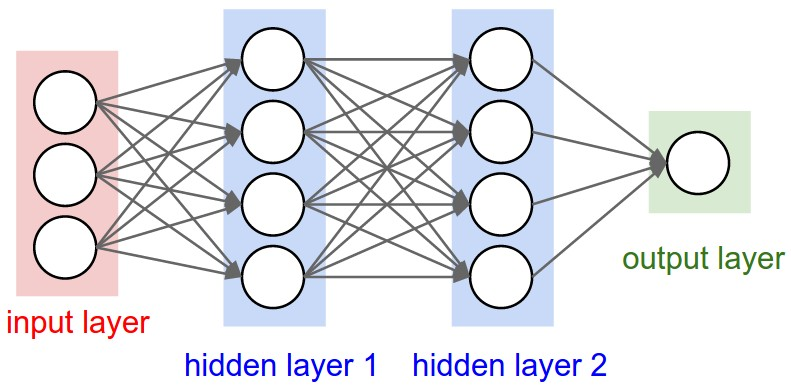
\includegraphics[width=0.48\textwidth]{mlearn_neural_network}
	}
	\hfill
	\subfloat[]
	{
		\label{fig:subfig:mlearn_cnn}
		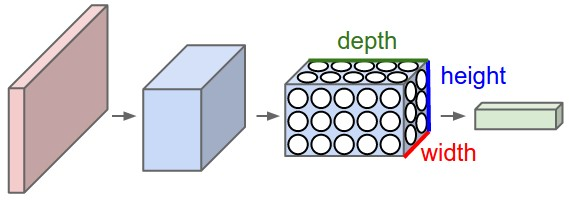
\includegraphics[width=0.48\textwidth]{mlearn_cnn}
	}
	\caption[Regular Neural Networks and Convolutional Neural Networks]{\textbf{(a)} Fully-connected neural network where each neuron of a layer is connected to every neuron of the previous layer. \textbf{(b)} CNN where the weights are organized in a \gls{3d} way. Each of the nodes is only locally connected to nodes of the previous layer. The main motivation behind this is that a learned filter (e.g. edge detector) is useful over the whole image. Images from~\cite{KarpathyStanfordRecognition}.}
	\label{fig:mlearn_nn_cnn}  
\end{figure}


\begin{figure}[htbp]
    \centering
	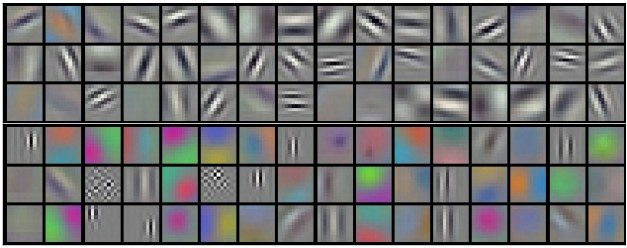
\includegraphics[width=0.8\textwidth]{mlearn_weights}
    \caption[Learned Weights of a trained AlexNet]{Learned convolutional filters of the first layer of an AlexNet trained for natural image classification~\cite{Krizhevsky2012ImageNetNetworks}. The learned filters act as detectors for high-frequency gray-scale features, mostly edges, and low-frequency color features.}
    \label{fig:mlearn_weights}
\end{figure}

\section{Related Work} % =================================================================================
As of today, there is relatively low interest from the scientific community in the segmentation of the nerves of the \gls{pns}. Felisaz et al.\cite{Felisaz2016NerveMicro-neurography} proposed a semi-automatic method to segment and measure the volumes of different compartments of the tibial nerve based on \gls{mrn} images. They measured fascicular volume, epineural volume, nerve volume, and the \gls{fnr}. They also calculated the inter- and intra-observer agreements. They concluded that the method is reproducible and \gls{fnr} is a novel biomarker, which may help in the diagnosis of peripheral neuropathies.
In \cite{Felisaz2017MRNeuropathy.} they further studied the assessment of morphometric ultrastructural changes in nerves affected by diabetic peripheral neuropathy. As in their previous work, they used a semi-automated technique of tissue segmentation to calculate nerve volumes, fascicle volumes, the \gls{fnr}, and the \gls{csa}. They noted increased nerve volumes and decreased \gls{fnr} in patients with diabetic peripheral neuropathy. The fascicle volume was increased in patients with moderate to severe diabetic peripheral neuropathy.
In their recently published work \cite{FelisazTextureNeuropathy} they applied texture analysis to MRN images and concluded that texture analysis might help to discriminate between normal and pathologic nerves.\\
Balsiger et al. investigated the use of hand-crafted features for the semi-automatic segmentation of the peripheral nerves with \gls{rf}. The \gls{rf}, was trained in a supervised fashion on hand-crafted features on a dataset consisting of \gls{mrn} images. Besides intensity-based features, the approach also incorporated a context feature. For this context feature, the user annotated the centers of the proximal and distal ends of the sciatic nerve by a single voxel in the MRN image. In case the branching of the sciatic nerve is included in the MRN image, the user annotated additionally its location. The nerve centers for the non-annotated slices were interpolated via first-order B-spline. The final context feature was obtained by the Euclidean distance from each pixel to the center of the nerve in each slice. Although the user annotation was limited, the clinical adoption of this approach is still questionable due to the user interaction. Motivated by the issue, their recent work~\cite{Balsiger2018SegmentationApproach} included a  fully-automatic deep learning-based method to segment the peripheral nerves. A \gls{fcnn} based on the fully-convolutional DenseNet~\cite{Huang2017DenselyNetworks} was trained on MRN images and evaluated. They achieved partial human-level performance compared to an inter-rater variability study. However, their approach based on a \gls{2d} \gls{fcnn} approach, which might be questionable due to the most recent advancements in medical image segmentation regarding \gls{3d} segmentation approaches. 

\section{Hypothesis} % ===================================================================================
Quantitative biomarkers for peripheral neuropathies, such as \gls{csa} and the \gls{fnr}, require an accurate segmentation of the peripheral nerve. Because manual segmentation is clinically unfeasible, computer-assisted segmentation is preferred.
For this reason, we aim to segment the sciatic nerve of the \gls{pns} fully-automatically from \acrshort{mrn} images, using a deep learning-based approach. Therefore, our first hypothesis is\\

\textit{Deep learning-based segmentation of peripheral nerves from \gls{mrn} images is possible with human-level performance.} \\

MRN images are \gls{3d} and the sciatic nerve is a \gls{3d} structure. Hence, our second hypothesis is\\

\textit{\gls{3d}-contextual information increases the segmentation accuracy.}

\section{Aim \& Structure of the Thesis} % ===============================================================
The aim of the thesis was to develop a deep learning-based approach to segment the sciatic nerve from \gls{mrn} images and to investigate the impact of \gls{3d} context on the segmentation performance.\\
\begin{itemize}
    \item Chapter~\ref{chap:methods} presents the used materials and the developed methods. It elaborates on how we designed and trained our neural networks, dealt with the problem of overfitting, and how we applied post-processing. Furthermore, the conducted experiments are defined.
    \item Chapter~\ref{chap:results} presents the obtained results for the proposed experiments. Further detailed results can be found in Appendix~\ref{app:results}.
    \item Chapter~\ref{chap:discussion_and_conclusions} discusses the results and conclusions are drawn.
    \item Chapter~\ref{chap:outlook} presents a visionary outlook.
\end{itemize}

\endinput